%% ============================================================
%% Applying OAuth 2.1 Token Exchange with Nested Actor Claims
%% to MCP Agentic Workflows
%% v4 — TikZ sequence diagrams, fixed layouts, fixed equation
%%
%% Compile: pdflatex (run twice for cross-references)
%% Packages: IEEEtran (journal), tikz, pgfplots,
%%           booktabs, multirow, colortbl, tabularx,
%%           amsmath (multline)
%% ============================================================
\documentclass[journal]{IEEEtran}
\IEEEoverridecommandlockouts

\usepackage{cite}
\usepackage{amsmath,amssymb,amsfonts}
\usepackage{graphicx}
\usepackage{textcomp}
\usepackage{xcolor}
\usepackage{booktabs}
\usepackage{url}
\usepackage{hyperref}
\usepackage{listings}
\usepackage{multirow}
\usepackage{array}
\usepackage{tikz}
\usepackage{pgfplots}
\usepackage{colortbl}
\usepackage{tabularx}
\usepackage{balance}

\usetikzlibrary{
  arrows.meta, shapes, positioning, fit,
  backgrounds, calc, decorations.pathreplacing,
  decorations.text
}
\pgfplotsset{compat=1.18}

\hypersetup{colorlinks=true,linkcolor=blue,citecolor=blue,urlcolor=blue}

%% ── colour palette ──────────────────────────────────────────
\definecolor{C_BASE}{HTML}{E07B54}  % warm orange – insecure / baseline
\definecolor{C_SEC} {HTML}{4C9BE8}  % cool blue   – NAC / secure
\definecolor{C_PAR} {HTML}{5DBB7A}  % green       – blocked / parallel
\definecolor{C_WARN}{HTML}{E74C3C}  % red         – attack / warning
\definecolor{C_HEAD}{HTML}{2C3E50}  % dark navy   – headers
\definecolor{SD_BG} {HTML}{EBF4FF}  % light blue  – sequence actor bg

%% ── code listing style ──────────────────────────────────────
\lstset{
  basicstyle=\scriptsize\ttfamily,
  breaklines=true,
  frame=single,
  captionpos=b,
  xleftmargin=1.2em,
  numbers=left,
  numberstyle=\tiny\color{gray},
  numbersep=4pt,
}

%% ── global TikZ styles ──────────────────────────────────────
\tikzset{
  %% -- sequence diagram actors --
  SD/actor/.style={
    draw=C_HEAD!60, rounded corners=3pt,
    fill=SD_BG, minimum width=2.3cm, minimum height=0.58cm,
    align=center, font=\scriptsize\bfseries
  },
  %% -- sequence diagram lifeline --
  SD/life/.style={draw, dashed, gray!55, thin},
  %% -- sequence diagram forward arrow --
  SD/fwd/.style={-{Stealth[length=3.5pt]}, thick, color=C_HEAD!80},
  %% -- sequence diagram response arrow --
  SD/bck/.style={-{Stealth[length=3.5pt]}, thick, dashed, color=gray!65},
  %% -- sequence diagram message label --
  SD/lbl/.style={font=\tiny, fill=white, inner sep=1.5pt, align=center},
  %% -- sequence diagram "par" combined fragment --
  SD/par/.style={draw=gray, dashed, thick, rounded corners=2pt},
  %% -- generic box (architecture diagrams) --
  arch/hub/.style={
    draw, rounded corners=4pt, fill=C_SEC!18,
    minimum width=1.9cm, minimum height=0.6cm,
    align=center, font=\scriptsize\bfseries
  },
  arch/worker/.style={
    draw, rounded corners=4pt, fill=C_PAR!22,
    minimum width=1.6cm, minimum height=0.55cm,
    align=center, font=\scriptsize
  },
  arch/oauth/.style={
    draw, rounded corners=4pt, fill=C_BASE!18,
    minimum width=1.9cm, minimum height=0.6cm,
    align=center, font=\scriptsize\bfseries
  },
  arch/user/.style={
    draw, rounded corners=4pt, fill=gray!14,
    minimum width=1.4cm, minimum height=0.55cm,
    align=center, font=\scriptsize\bfseries
  },
  arch/arr/.style={-{Stealth[length=3.5pt]}, thick},
  arch/darr/.style={-{Stealth[length=3.5pt]}, thick, dashed, gray!70},
}

%% ============================================================
\begin{document}

\title{Applying OAuth 2.1 Token Exchange with Nested Actor Claims\\
to MCP Agentic Workflows:\\
An Architectural Pattern for Secure Delegation}

\author{\IEEEauthorblockN{[Author Name]}
\IEEEauthorblockA{\textit{[Department]} \\
\textit{[Institution]}\\
[City, Country]\\
[email@institution.edu]}}

\maketitle

%% ============================================================
\begin{abstract}
The Model Context Protocol (MCP) has emerged as the standard interface for
connecting large language model (LLM) agents to downstream tool services.
As deployments scale to multi-service orchestration, a pervasive security
anti-pattern has become prevalent: \textit{token passthrough}, in which an
orchestrating AI assistant forwards the user's original OAuth access token
unchanged to every downstream service it invokes. We demonstrate that this
practice simultaneously violates three independent security properties---audience
binding, scope attenuation, and delegation chain visibility---collectively
constituting the \textit{Confused Deputy Problem} as identified in the MCP
security specification.

We propose an architectural pattern based on RFC 8693 (OAuth 2.0 Token Exchange)
with Nested Actor Claims (NAC) as a principled, standards-compliant solution.
Under this pattern, an orchestrator exchanges the parent token for a fresh child
token at each delegation hop; each child token carries a service-specific audience
claim, an attenuated scope, a nested \texttt{act} claim recording the delegation
chain, and a one-time-use identifier preventing replay. The pattern is
authorization-server-agnostic and can be adopted by any conforming OAuth~2.1
deployment regardless of implementation language or platform.

We present an empirical evaluation against four concrete attack vectors---scope
escalation, lateral movement, token replay, and identity confusion. Results from
30 experimental trials per scenario demonstrate a 100\% attack block rate in all
cases. An ablation study of 720 trials across six enforcement configurations
confirms that each security property is independently necessary. Per-hop
cryptographic overhead is bounded at approximately 3--5\,ms (one RSA-2048 signing
operation plus one revocation store update), yielding $O(k)$ total overhead for a
$k$-hop delegation chain. Production deployment overhead is projected at
$+7$--$15\%$ relative to the insecure baseline. These results demonstrate that the
RFC~8693 NAC pattern provides provable, measurable, and deployable security for
MCP agentic workflows at acceptable production cost.
\end{abstract}

\begin{IEEEkeywords}
Model Context Protocol, OAuth 2.1, RFC 8693, Token Exchange, Nested Actor Claims,
Confused Deputy, Multi-Agent AI, Delegation Chain, Agentic Security, OWASP GenAI
\end{IEEEkeywords}

%% ============================================================
\section{Introduction}
\label{sec:introduction}
%% ============================================================

Autonomous AI systems are rapidly transitioning from single-model assistants to
distributed multi-agent orchestrators. A user asks an AI assistant to
``review my calendar, summarise the relevant notes, send the summary by email, and
post an update to the team channel.'' Behind this single natural-language request
lies a coordinated sequence of calls to four distinct downstream services, each
with its own authorization requirements.

The Model Context Protocol (MCP) \cite{mcp_spec}, introduced by Anthropic in
November 2024 and subsequently adopted across the industry, provides the emerging
standard interface for this hub-and-spoke architecture: an \textit{assistant hub}
receives tool calls from an agent and in turn calls \textit{worker services} as
an HTTP client. This intermediary role creates an authorization challenge. The
user delegates authority to the hub by providing an OAuth access token. The hub
must somehow convey appropriate authorization to each downstream worker.

The natural, default approach is \textbf{token passthrough}: the hub forwards the
original user token unchanged to every service it calls. This approach is
functionally correct---services respond and the workflow completes---but it is
deeply insecure. The MCP security specification \cite{mcp_security} explicitly
identifies token passthrough as an \textit{anti-pattern} that ``creates confused
deputy risks,'' and the Coalition for Secure AI (CoSAI) whitepaper on MCP
security \cite{cosai_mcp} states: ``don't pass through OAuth tokens directly.
Use token exchange (RFC 8693) to maintain full accountability and prevent confused
deputy attacks.''

Despite this consensus recommendation, no prior work has (1)~formally
characterised the three security properties that token passthrough violates,
(2)~described an architectural pattern for remediation that is
implementation-agnostic, (3)~provided an ablation study demonstrating the
independent necessity of each property, and (4)~empirically quantified the
overhead of the remediated pattern. This paper addresses all four gaps.

\textbf{Contributions:}
\begin{enumerate}
  \item We formally characterise the token passthrough anti-pattern and the three
        independent security properties it violates
        (Section~\ref{sec:problem}).
  \item We propose the \textit{RFC 8693 NAC architectural pattern} for MCP
        multi-agent delegation and prove it satisfies all three properties by
        construction (Section~\ref{sec:solution}).
  \item We present a reference implementation and evaluate it against four
        concrete attack vectors with a 720-trial ablation study confirming
        property independence (Section~\ref{sec:eval}).
  \item We derive theoretical bounds on per-hop overhead and validate them
        empirically (Section~\ref{sec:eval}).
\end{enumerate}

%% ============================================================
\section{Background and Definitions}
\label{sec:background}
%% ============================================================

\subsection{Large Language Models and Agentic Systems}

A \textit{Large Language Model} (LLM) is a neural network trained to generate
text conditioned on a prompt \cite{vaswani2017}. Modern LLMs exhibit emergent
capabilities including multi-step reasoning and tool use. \textit{Agentic AI}
refers to systems in which an LLM autonomously selects and executes actions to
achieve user-specified goals \cite{wang2024survey}. The \textit{ReAct} paradigm
\cite{yao2022react} interleaves reasoning with action calls: the model reasons
about which tool to invoke, calls it, observes the result, and re-plans. This
is the computational model underlying MCP tool use.

\subsection{The Model Context Protocol}

MCP \cite{mcp_spec} defines a client-server protocol over JSON-RPC 2.0. An
\textit{MCP server} exposes \textit{tools} (callable functions), \textit{resources}
(data), and \textit{prompts} (templates) to an \textit{MCP client}. Authentication
is carried via the \texttt{Authorization: Bearer} HTTP header.

The MCP authorization specification \cite{mcp_spec_2025} treats MCP servers as
OAuth 2.1 resource servers. Figure~\ref{fig:mcp_std_auth} shows the standard
authorization flow: the MCP client discovers the authorization server via
Protected Resource Metadata (PRM), performs an OAuth 2.1 authorization code flow
with PKCE, obtains an access token, and uses it to call the MCP server. This flow
governs the \textit{client-to-hub} boundary only. It does not specify how the hub
should authorize its own calls to downstream worker services---the gap this paper
fills.

\begin{figure*}[t]
\centering
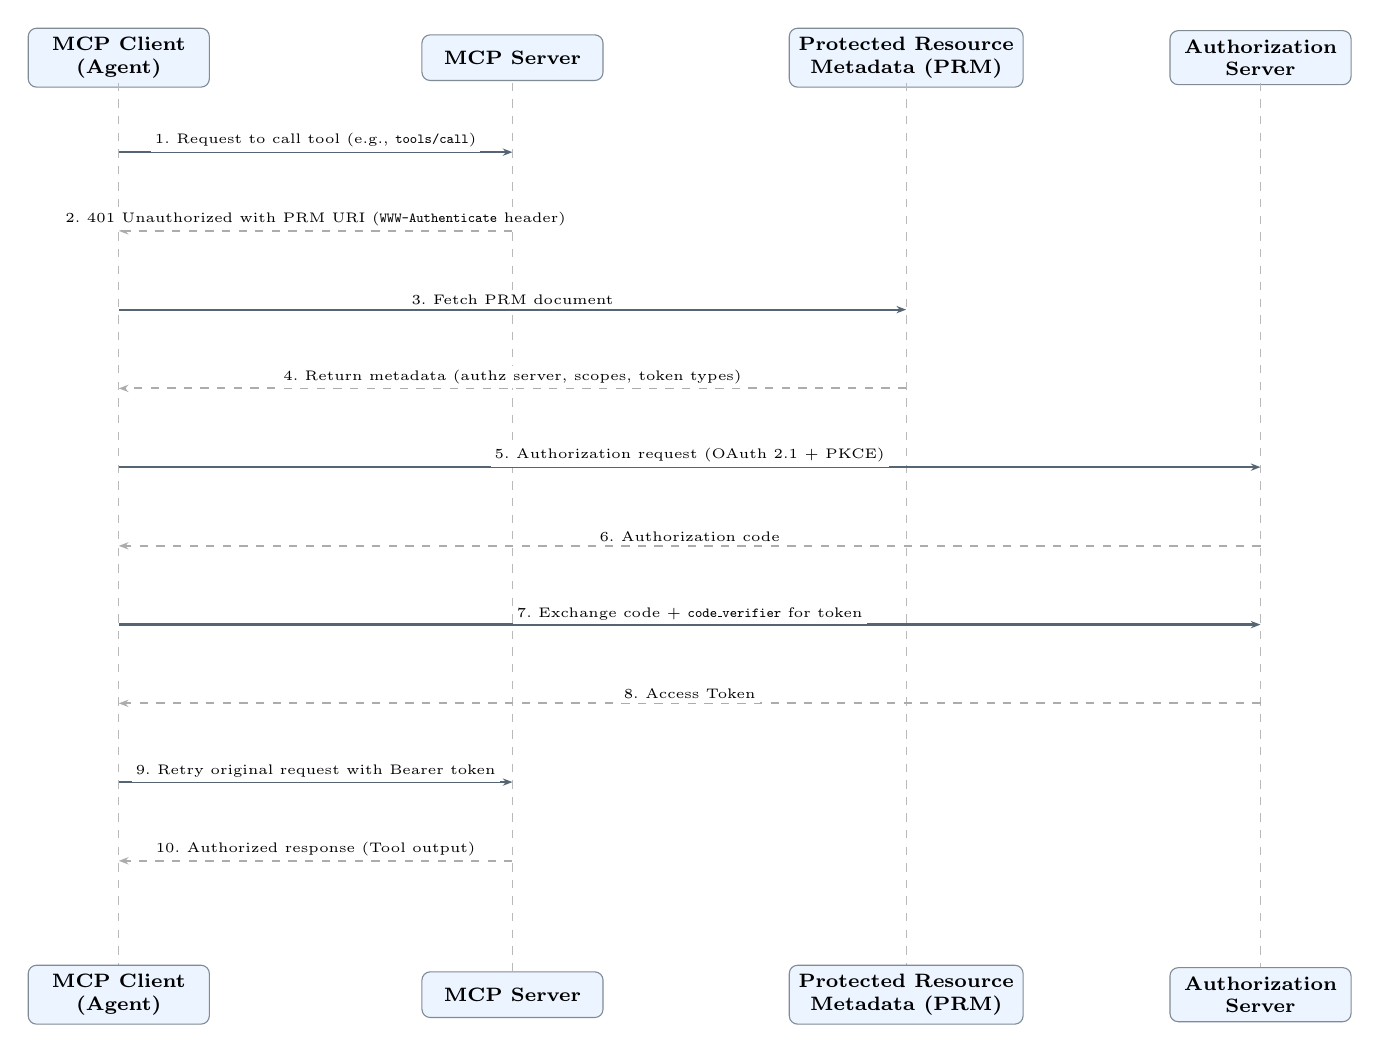
\begin{tikzpicture}[
  every node/.style={font=\scriptsize},
  x=1cm, y=1cm,
]
%% ── Actor x-positions ────────────────────────────────────────
%% textwidth ≈ 17cm; 4 actors, each 2.4cm wide, centred as below
\pgfmathsetmacro{\xC}{1.8}   % MCP Client
\pgfmathsetmacro{\xS}{6.8}   % MCP Server
\pgfmathsetmacro{\xP}{11.8}  % PRM
\pgfmathsetmacro{\xA}{16.3}  % Auth Server

%% ── Top actor boxes ──────────────────────────────────────────
\node[SD/actor, minimum width=2.3cm] (C1) at (\xC, 0)
  {MCP Client\\(Agent)};
\node[SD/actor, minimum width=2.3cm] (S1) at (\xS, 0)
  {MCP Server};
\node[SD/actor, minimum width=2.8cm] (P1) at (\xP, 0)
  {Protected Resource\\Metadata (PRM)};
\node[SD/actor, minimum width=2.3cm] (A1) at (\xA, 0)
  {Authorization\\Server};

%% ── Lifelines ────────────────────────────────────────────────
\draw[SD/life] (\xC,-0.32) -- (\xC,-11.6);
\draw[SD/life] (\xS,-0.32) -- (\xS,-11.6);
\draw[SD/life] (\xP,-0.32) -- (\xP,-11.6);
\draw[SD/life] (\xA,-0.32) -- (\xA,-11.6);

%% ── Messages ─────────────────────────────────────────────────
%% 1. Client → Server  (solid)
\draw[SD/fwd] (\xC,-1.2) -- (\xS,-1.2);
\node[SD/lbl, above] at ({(\xC+\xS)/2},-1.2)
  {1.\ Request to call tool (e.g., \texttt{tools/call})};

%% 2. Server → Client  (dashed, 401)
\draw[SD/bck] (\xS,-2.2) -- (\xC,-2.2);
\node[SD/lbl, above] at ({(\xC+\xS)/2},-2.2)
  {2.\ 401 Unauthorized with PRM URI (\texttt{WWW-Authenticate} header)};

%% 3. Client → PRM  (solid)
\draw[SD/fwd] (\xC,-3.2) -- (\xP,-3.2);
\node[SD/lbl, above] at ({(\xC+\xP)/2},-3.2)
  {3.\ Fetch PRM document};

%% 4. PRM → Client  (dashed)
\draw[SD/bck] (\xP,-4.2) -- (\xC,-4.2);
\node[SD/lbl, above] at ({(\xC+\xP)/2},-4.2)
  {4.\ Return metadata (authz server, scopes, token types)};

%% 5. Client → Auth  (solid)
\draw[SD/fwd] (\xC,-5.2) -- (\xA,-5.2);
\node[SD/lbl, above] at ({(\xC+\xA)/2},-5.2)
  {5.\ Authorization request (OAuth 2.1 + PKCE)};

%% 6. Auth → Client  (dashed)
\draw[SD/bck] (\xA,-6.2) -- (\xC,-6.2);
\node[SD/lbl, above] at ({(\xC+\xA)/2},-6.2)
  {6.\ Authorization code};

%% 7. Client → Auth  (solid)
\draw[SD/fwd] (\xC,-7.2) -- (\xA,-7.2);
\node[SD/lbl, above] at ({(\xC+\xA)/2},-7.2)
  {7.\ Exchange code + \texttt{code\_verifier} for token};

%% 8. Auth → Client  (dashed)
\draw[SD/bck] (\xA,-8.2) -- (\xC,-8.2);
\node[SD/lbl, above] at ({(\xC+\xA)/2},-8.2)
  {8.\ Access Token};

%% 9. Client → Server  (solid)
\draw[SD/fwd] (\xC,-9.2) -- (\xS,-9.2);
\node[SD/lbl, above] at ({(\xC+\xS)/2},-9.2)
  {9.\ Retry original request with Bearer token};

%% 10. Server → Client  (dashed)
\draw[SD/bck] (\xS,-10.2) -- (\xC,-10.2);
\node[SD/lbl, above] at ({(\xC+\xS)/2},-10.2)
  {10.\ Authorized response (Tool output)};

%% ── Bottom actor boxes (UML convention) ──────────────────────
\node[SD/actor, minimum width=2.3cm] at (\xC,-11.9)
  {MCP Client\\(Agent)};
\node[SD/actor, minimum width=2.3cm] at (\xS,-11.9)
  {MCP Server};
\node[SD/actor, minimum width=2.8cm] at (\xP,-11.9)
  {Protected Resource\\Metadata (PRM)};
\node[SD/actor, minimum width=2.3cm] at (\xA,-11.9)
  {Authorization\\Server};

\end{tikzpicture}
\caption{Standard MCP OAuth 2.1 + PKCE authorization flow (UML sequence
diagram). The MCP client discovers the authorization server via Protected
Resource Metadata, performs the OAuth 2.1 PKCE authorization code flow, and
obtains an access token. Solid arrows are requests; dashed arrows are
responses. Critically, \textbf{this flow covers only the client-to-hub
authorization boundary}. How the hub authorizes its own calls to downstream
worker services is unspecified---the delegation security gap this paper
addresses.}
\label{fig:mcp_std_auth}
\end{figure*}

In multi-service deployments, the AI assistant hub acts as both an MCP server
(receiving tool calls from the agent) and an HTTP client (calling downstream
worker services). This dual role is the hub-and-spoke topology that the MCP
security specification identifies as the confused deputy attack surface.

\subsection{OAuth 2.1 and Bearer Tokens}

OAuth 2.1 \cite{oauth21} is the current revision of the OAuth 2.0 authorization
framework \cite{rfc6749}, mandating PKCE for all public clients and deprecating
the implicit grant. An \textit{access token} is a bearer credential encoding the
authorized subject (\texttt{sub}), audience (\texttt{aud}), and permission set
(\texttt{scope}).

RFC 9068 \cite{rfc9068} profiles access tokens as signed JSON Web Tokens (JWTs)
\cite{rfc7519}. JWT claims relevant to this work are:
\begin{itemize}
  \item \textbf{\texttt{aud}}: the intended recipient(s); a receiver MUST reject
        tokens not intended for it \cite{rfc9068};
  \item \textbf{\texttt{scope}}: the set of permissions the token carries;
  \item \textbf{\texttt{jti}}: a unique identifier for the token, enabling
        revocation and replay prevention;
  \item \textbf{\texttt{act}}: the actor claim (RFC 8693), recording the identity
        of the party exercising delegated authority.
\end{itemize}

\subsection{RFC 8693: OAuth 2.0 Token Exchange}

RFC 8693 \cite{rfc8693} defines an HTTP Security Token Service (STS) protocol
for exchanging one token for another with different properties. The specification
defines two delegation semantics:

\textbf{Impersonation}: The acting party takes on the full identity of the
subject; the intermediate is invisible to downstream services.

\textbf{Delegation}: The acting party remains distinguishable from the subject.
The new token retains the subject identity while recording the actor in the
\texttt{act} claim. For agentic workflows, delegation is the appropriate
choice---the user identity ($\texttt{sub}$) is preserved for accountability while
the orchestrating agent is recorded as the actor.

RFC 8693 defines the scope non-escalation invariant: the requested scope of a
derived token must not exceed that of the subject token. This is the formal
basis for scope attenuation enforcement. The specification also defines the
nesting semantics for the \texttt{act} claim:

\begin{lstlisting}[language={},caption={Nested act claim per RFC 8693 \S 4.1},
                   label={lst:actchain}]
{
  "sub": "alice",
  "aud": "service-B",
  "act": {
    "sub": "orchestrator",
    "act": {
      "sub": "prior-actor"  // chain grows inward
    }
  }
}
\end{lstlisting}

RFC 8693 is deployed in production by Microsoft (On-Behalf-Of flow), Auth0
(Token Vault), ZITADEL, Authlete, Keycloak, Box, Salesforce, and
RedHat \cite{rfc8693_deploy}.

\subsection{Token Revocation Stores}

RFC 7009 \cite{rfc7009} defines OAuth 2.0 token revocation. For per-request
one-time-use semantics---where a token's \texttt{jti} must be revoked after a
single use---the revocation check must be cross-process and low-latency. The
canonical architecture is an in-memory key-value store with TTL-based expiry:
the record is written after issuance (\textit{register}), queried before each
use (\textit{check}), and overwritten after consumption (\textit{revoke}). Any
implementation satisfying this interface---whether managed (e.g., AWS
ElastiCache, Google Memorystore) or self-hosted (e.g., Redis, DragonflyDB)---
satisfies the requirement. The specific technology choice affects operational
latency and availability, not security semantics.

\subsection{OWASP Generative AI Top 10 (2025)}

The OWASP Top 10 for Large Language Model Applications 2025 \cite{owasp_genai}
identifies the most critical LLM security risks. Relevant to this work:
\begin{itemize}
  \item \textbf{LLM06:2025 Excessive Agency}: Agents granted more permissions
        or capability than their task requires---the root cause of the scope
        escalation attack vector.
  \item \textbf{LLM01:2025 Prompt Injection}: Attacker-controlled input causing
        an agent to exercise legitimately authorized tokens in unauthorised ways,
        amplified when tokens carry excess scopes.
\end{itemize}


%% ============================================================
\section{Problem Statement}
\label{sec:problem}
%% ============================================================

\subsection{The Token Passthrough Anti-Pattern}

Let $\mathcal{H}$ denote the assistant hub, $\mathcal{W}=\{W_1,\ldots,W_n\}$ the
set of downstream worker services, $u$ the authenticated user, and $\mathcal{A}$
the OAuth authorization server. $\mathcal{A}$ issues a root access token:

\begin{equation}
T_0 = \mathrm{JWT}\!\left(\begin{array}{l}
  \texttt{sub} = u,\quad \texttt{aud} = \mathcal{H},\\[2pt]
  \texttt{scope} = S_0 = \textstyle\bigcup_{i}\, s_i,\quad
  \texttt{jti} = j_0
\end{array}\right)
\label{eq:root}
\end{equation}

where $S_0$ is the union of all scopes required by any worker. In the token
passthrough pattern, $\mathcal{H}$ forwards $T_0$ unchanged to every worker:

\begin{equation}
\mathrm{call}(W_i,\; T_0) \quad \forall\, i \in \{1, \ldots, n\}
\label{eq:passthrough}
\end{equation}

Figure~\ref{fig:passthrough} visualises this topology.

%% ---- FIGURE 2: Token Passthrough Architecture ----
\begin{figure}[t]
\centering
\resizebox{\columnwidth}{!}{%
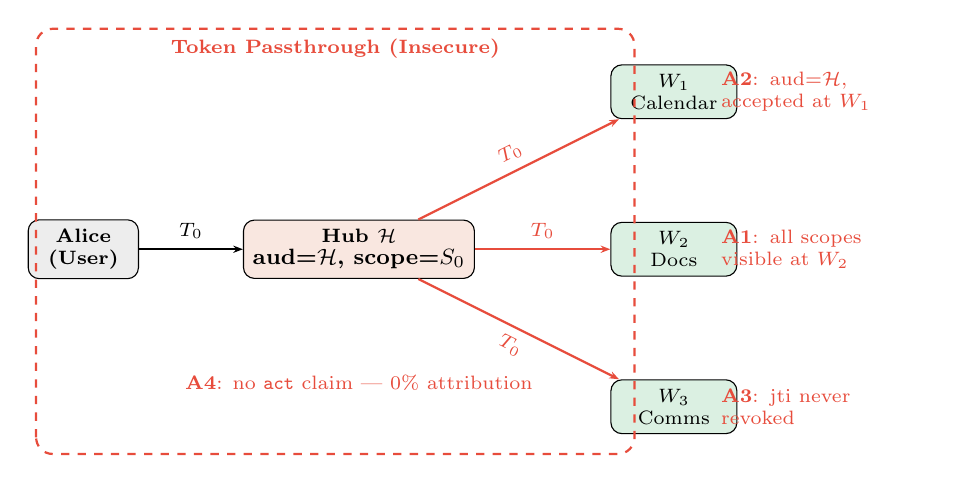
\begin{tikzpicture}[
  every node/.style={font=\small},
  x=1cm, y=1cm,
]
%% Nodes
\node[arch/user]  (alice) at (0, 2.5)   {Alice\\(User)};
\node[arch/oauth] (hub)   at (3.5, 2.5)
  {Hub $\mathcal{H}$\\{\footnotesize aud=$\mathcal{H}$, scope=$S_0$}};
\node[arch/worker](w1)    at (7.5, 4.5)  {$W_1$\\Calendar};
\node[arch/worker](w2)    at (7.5, 2.5)  {$W_2$\\Docs};
\node[arch/worker](w3)    at (7.5, 0.5)  {$W_3$\\Comms};

%% Alice → Hub
\draw[arch/arr] (alice) -- node[above,font=\scriptsize]{$T_0$} (hub);

%% Hub → Workers (same token)
\draw[arch/arr, color=C_WARN]
  (hub) -- node[above,sloped,font=\scriptsize]{$T_0$} (w1);
\draw[arch/arr, color=C_WARN]
  (hub) -- node[above,font=\scriptsize]{$T_0$} (w2);
\draw[arch/arr, color=C_WARN]
  (hub) -- node[below,sloped,font=\scriptsize]{$T_0$} (w3);

%% Attack annotations (below each arrow, right side)
\node[font=\scriptsize, color=C_WARN, text width=2.6cm, align=left]
  at (9.4, 4.5)
  {\textbf{A2}: aud=$\mathcal{H}$,\\accepted at $W_1$};
\node[font=\scriptsize, color=C_WARN, text width=2.6cm, align=left]
  at (9.4, 2.5)
  {\textbf{A1}: all scopes\\visible at $W_2$};
\node[font=\scriptsize, color=C_WARN, text width=2.6cm, align=left]
  at (9.4, 0.5)
  {\textbf{A3}: jti never\\revoked};

%% A4 annotation under hub
\node[font=\scriptsize, color=C_WARN, align=center]
  at (3.5, 0.8)
  {\textbf{A4}: no \texttt{act} claim — 0\% attribution};

%% Border box indicating vulnerability
\draw[draw=C_WARN, dashed, thick, rounded corners=6pt]
  (-0.6, -0.1) rectangle (7.0, 5.3);
\node[font=\scriptsize\bfseries, color=C_WARN] at (3.2, 5.05)
  {Token Passthrough (Insecure)};
\end{tikzpicture}
}
\caption{Token passthrough anti-pattern: the hub forwards $T_0$ (with
hub-bound audience and full scope $S_0$) \emph{unchanged} to every worker,
simultaneously enabling all four attacks (A1--A4).}
\label{fig:passthrough}
\end{figure}

\subsection{Three Violated Security Properties}

\begin{definition}[\textbf{Audience Binding, P1}]
A token $T$ satisfies audience binding for worker $W_i$ iff
$\mathrm{aud}(T) = \mathrm{AUDIENCE}(W_i)$.
\end{definition}

\textbf{Violation:} $T_0$ carries $\texttt{aud} = \mathcal{H}$. When presented
to $W_i \neq \mathcal{H}$, RFC~9068 requires rejection. In practice, many
implementations omit this check.

\begin{definition}[\textbf{Scope Attenuation, P2}]
A token $T$ satisfies scope attenuation for $W_i$ iff
$\mathrm{scope}(T) \subseteq s_i$, where $s_i$ is the minimum scope $W_i$
requires to execute its function.
\end{definition}

\textbf{Violation:} $T_0$ carries $S_0 = \bigcup_j s_j$. Worker $W_i$ receives
permissions intended for every other service, violating least privilege. A
compromised $W_i$ inherits the full authority of the system.

\begin{definition}[\textbf{Delegation Chain Visibility, P3}]
A token $T$ satisfies chain visibility iff the \texttt{act} claim of $T$
contains a cryptographically verifiable record of every agent that handled $T$
on behalf of subject $u$.
\end{definition}

\textbf{Violation:} $T_0$ carries no \texttt{act} claim. Every audit record
contains only $\texttt{sub} = u$. Calls originating from different agents are
indistinguishable in the audit trail.

\subsection{The Confused Deputy Problem in MCP}

Hardy's 1988 analysis \cite{hardy1988} applies directly:

\begin{itemize}
  \item \textbf{Principal}: User $u$, who delegated authority $T_0$ to
        $\mathcal{H}$.
  \item \textbf{Deputy}: Hub $\mathcal{H}$, which holds $T_0$ and calls workers.
  \item \textbf{Confused action}: $\mathcal{H}$ presents $T_0$ to $W_i$, where
        it carries capabilities $u$ never intended for $W_i$.
  \item \textbf{Adversary}: Any agent or prompt injection that exploits the
        excess authority in $T_0$.
\end{itemize}

The MCP specification \cite{mcp_security} states: ``Servers SHOULD NOT pass
tokens received from clients to other servers, as this creates confused deputy
risks.''

\subsection{Four Concrete Attack Vectors}

\begin{table}[h]
\caption{Formal attack vector definitions}
\label{tab:attack_formal}
\centering
\footnotesize
\setlength{\tabcolsep}{3pt}
\begin{tabularx}{\columnwidth}{l X c}
\toprule
\textbf{ID} & \textbf{Mechanism} & \textbf{Requires} \\
\midrule
A1 & Agent calls a privileged tool using a token without the required scope
     & $\neg$\,P2 \\
A2 & Token obtained for service $W_i$ is replayed at $W_j\;(i\neq j)$
     & $\neg$\,P1 \\
A3 & Captured child token is replayed for a second unauthorised call
     & No revocation \\
A4 & Audit log lacks delegation chain; calls cannot be attributed to agent
     & $\neg$\,P3 \\
\bottomrule
\end{tabularx}
\end{table}


%% ============================================================
\section{The RFC 8693 NAC Architectural Pattern}
\label{sec:solution}
%% ============================================================

\subsection{Pattern Overview}

Before invoking worker $W_i$, the orchestrating hub presents its current token
to the authorization server's token exchange endpoint and obtains a fresh,
narrowly scoped child token:

\begin{equation}
T_i = \mathrm{Exchange}\!\left(
  T_{\mathrm{parent}},\;
  \mathrm{AUDIENCE}(W_i),\;
  s_i,\;
  \mathcal{H}
\right)
\label{eq:exchange}
\end{equation}

where $T_i$ is constructed by the authorization server as:

\begin{equation}
T_i = \mathrm{JWT}\!\left(\begin{array}{l}
  \texttt{sub} = u, \\[2pt]
  \texttt{aud} = \mathrm{AUDIENCE}(W_i), \\[2pt]
  \texttt{scope} = s_i \;\subseteq\; \mathrm{scope}(T_{\mathrm{parent}}), \\[2pt]
  \texttt{jti} = j_i \;\text{(fresh, unique)}, \\[2pt]
  \texttt{act} = \{\,\texttt{sub}\text{:}\,\mathcal{H},\;
                    \texttt{act}\text{:}\,T_{\mathrm{parent}}.\texttt{act}\,\}
\end{array}\right)
\label{eq:child}
\end{equation}

This construction directly restores all three violated properties: the
\texttt{aud} satisfies P1, the scope satisfies P2, and the \texttt{act} chain
satisfies P3. Figure~\ref{fig:nac_arch} shows the NAC architecture, and
Figure~\ref{fig:nac_seq} illustrates the complete token exchange sequence.

%% ---- FIGURE 3: NAC Architecture (single column, fixed) ----
\begin{figure}[t]
\centering
\resizebox{\columnwidth}{!}{%
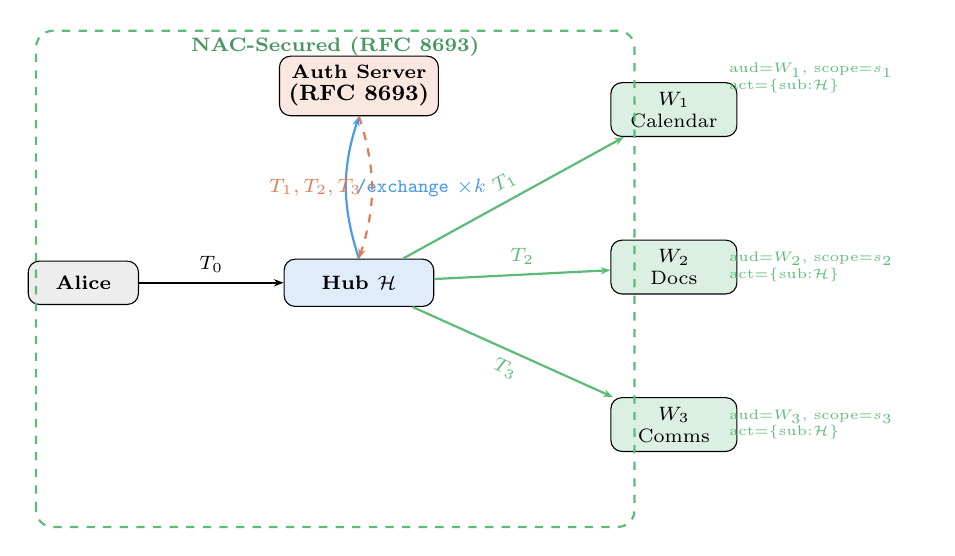
\begin{tikzpicture}[
  every node/.style={font=\small},
  x=1cm, y=1cm,
]
%% Nodes
\node[arch/user]  (alice)  at (0, 3.0)
  {Alice};
\node[arch/oauth] (auth)   at (3.5, 5.5)
  {Auth Server\\{\footnotesize(RFC 8693)}};
\node[arch/hub]   (hub)    at (3.5, 3.0)
  {Hub $\mathcal{H}$};
\node[arch/worker](w1)     at (7.5, 5.2)
  {$W_1$\\Calendar};
\node[arch/worker](w2)     at (7.5, 3.2)
  {$W_2$\\Docs};
\node[arch/worker](w3)     at (7.5, 1.2)
  {$W_3$\\Comms};

%% Alice → Hub
\draw[arch/arr] (alice) -- node[above,font=\scriptsize]{$T_0$} (hub);

%% Hub ↔ Auth Server (exchange)
\draw[arch/arr, color=C_SEC, bend left=18]
  (hub.north) to node[right,font=\scriptsize,pos=0.5]
    {\texttt{/exchange} $\times k$} (auth.south);
\draw[arch/darr, color=C_BASE, bend left=18]
  (auth.south) to node[left,font=\scriptsize,pos=0.5]
    {$T_1, T_2, T_3$} (hub.north);

%% Hub → Workers (different tokens, colour-coded)
\draw[arch/arr, color=C_PAR]
  (hub) -- node[above,sloped,font=\scriptsize]{$T_1$} (w1);
\draw[arch/arr, color=C_PAR]
  (hub) -- node[above,font=\scriptsize]{$T_2$} (w2);
\draw[arch/arr, color=C_PAR]
  (hub) -- node[below,sloped,font=\scriptsize]{$T_3$} (w3);

%% Token property labels next to workers
\node[font=\tiny, color=C_PAR, text width=2.4cm, align=left]
  at (9.4, 5.6)
  {aud=$W_1$, scope=$s_1$\\act=\{sub:$\mathcal{H}$\}};
\node[font=\tiny, color=C_PAR, text width=2.4cm, align=left]
  at (9.4, 3.2)
  {aud=$W_2$, scope=$s_2$\\act=\{sub:$\mathcal{H}$\}};
\node[font=\tiny, color=C_PAR, text width=2.4cm, align=left]
  at (9.4, 1.2)
  {aud=$W_3$, scope=$s_3$\\act=\{sub:$\mathcal{H}$\}};

%% Green border indicating security
\draw[draw=C_PAR, dashed, thick, rounded corners=6pt]
  (-0.6, -0.1) rectangle (7.0, 6.2);
\node[font=\scriptsize\bfseries, color=C_PAR!80!black]
  at (3.2, 6.0) {NAC-Secured (RFC 8693)};
\end{tikzpicture}
}
\caption{RFC 8693 NAC pattern: the hub exchanges the root token $T_0$ for
per-service child tokens at the authorization server before each worker call.
Each $T_i$ carries a unique \texttt{aud}, attenuated \texttt{scope}, and
nested \texttt{act} chain, satisfying P1--P3 simultaneously.}
\label{fig:nac_arch}
\end{figure}

\subsection{Concurrent Issuance for Multiple Workers}

Because child tokens for $W_1, W_2, \ldots, W_k$ are issued from the same parent
token and are mutually independent (different audience, different scope, no
ordering constraint), they can be issued concurrently:

\begin{multline}
(T_1, T_2, \ldots, T_k) = \\
\mathrm{ConcurrentExchange}\!\left(
  T_{\mathrm{root}},\;
  \bigl\{\,(\mathrm{aud}_i,\; s_i)\,\bigr\}_{i=1}^{k}
\right)
\label{eq:concurrent}
\end{multline}

Concurrent issuance reduces wall-clock time from $k \times t_{\mathrm{exchange}}$
to $\approx t_{\mathrm{exchange}}$ (the maximum across concurrent requests),
subject to authorization server capacity. This is the basis for the
``parallel estimate'' in Section~\ref{sec:eval}.

\subsection{N-Hop Delegation Chains}

For hierarchical delegation---where $W_i$ must itself call a further downstream
service---the pattern applies recursively:

\begin{equation}
T_k = \mathrm{Exchange}(T_{k-1},\;
  \mathrm{AUDIENCE}(W_k),\; s_k,\; W_{k-1})
\label{eq:nhop}
\end{equation}

The \texttt{act} claim grows by one level per hop, recording the complete
delegation history. A depth limit prevents unbounded chain growth or circular
references. We demonstrate a 3-hop chain:
$\text{alice} \to \mathcal{H} \to W_{\mathrm{cal}} \to W_{\mathrm{ext}}$.

\subsection{NAC Token Exchange Sequence}

Figure~\ref{fig:nac_seq} provides the full UML sequence diagram for the NAC
token exchange flow, showing how Alice's root token is transformed into
per-service child tokens before any worker is called, and how the \texttt{jti}
is revoked after each use.

%% ---- FIGURE 4: NAC Exchange Sequence Diagram (full width) ----
\begin{figure*}[t]
\centering
\begin{tikzpicture}[
  every node/.style={font=\scriptsize},
  x=1cm, y=1cm,
]
%% ── Actor x-positions ──────────────────────────────────────
%% 6 actors, textwidth ≈ 17cm
\pgfmathsetmacro{\xAl}{0.9}   % Alice
\pgfmathsetmacro{\xHu}{4.1}   % Hub
\pgfmathsetmacro{\xAu}{8.3}   % Auth Server
\pgfmathsetmacro{\xW1}{12.0}  % W1 Calendar
\pgfmathsetmacro{\xW2}{14.2}  % W2 Docs
\pgfmathsetmacro{\xW3}{16.4}  % W3 Comms

%% ── Top actor boxes ────────────────────────────────────────
\node[SD/actor, minimum width=2.0cm] at (\xAl,0)
  {Alice\\(User)};
\node[SD/actor, minimum width=2.0cm] at (\xHu,0)
  {Hub $\mathcal{H}$};
\node[SD/actor, minimum width=2.4cm] at (\xAu,0)
  {Auth Server\\(RFC 8693)};
\node[SD/actor, minimum width=1.6cm] at (\xW1,0)
  {$W_1$\\Calendar};
\node[SD/actor, minimum width=1.6cm] at (\xW2,0)
  {$W_2$\\Docs};
\node[SD/actor, minimum width=1.6cm] at (\xW3,0)
  {$W_3$\\Comms};

%% ── Lifelines ──────────────────────────────────────────────
\foreach \x in {\xAl,\xHu,\xAu,\xW1,\xW2,\xW3}
  \draw[SD/life] (\x,-0.32) -- (\x,-13.5);

%% ── Phase 1: Root token ────────────────────────────────────
%% 1. Alice → Hub: Bearer T0
\draw[SD/fwd] (\xAl,-1.0) -- (\xHu,-1.0);
\node[SD/lbl, above] at ({(\xAl+\xHu)/2},-1.0)
  {1.\ Bearer $T_0$ in \texttt{Authorization} header
   (aud=$\mathcal{H}$, scope=$S_0$)};

%% ── Phase 2: Concurrent RFC 8693 exchanges ─────────────────
%% "par" combined fragment box
\draw[SD/par] (\xHu-0.5,-1.7) rectangle (\xAu+0.6,-5.0);
\node[font=\tiny\bfseries, fill=white, anchor=north west]
  at (\xHu-0.5,-1.7) {par\ (concurrent)};

%% 2a. Hub → Auth: exchange for T1
\draw[SD/fwd, color=C_PAR!80!black] (\xHu,-2.2) -- (\xAu,-2.2);
\node[SD/lbl, above] at ({(\xHu+\xAu)/2},-2.2)
  {2a.\ \texttt{POST /token/exchange}
   (aud=$W_1$, scope=$s_1$, actor=$\mathcal{H}$)};

%% 2b. Hub → Auth: exchange for T2
\draw[SD/fwd, color=C_PAR!80!black] (\xHu,-3.1) -- (\xAu,-3.1);
\node[SD/lbl, above] at ({(\xHu+\xAu)/2},-3.1)
  {2b.\ \texttt{POST /token/exchange}
   (aud=$W_2$, scope=$s_2$, actor=$\mathcal{H}$)};

%% 2c. Hub → Auth: exchange for T3
\draw[SD/fwd, color=C_PAR!80!black] (\xHu,-4.0) -- (\xAu,-4.0);
\node[SD/lbl, above] at ({(\xHu+\xAu)/2},-4.0)
  {2c.\ \texttt{POST /token/exchange}
   (aud=$W_3$, scope=$s_3$, actor=$\mathcal{H}$)};

%% 3. Auth → Hub: T1, T2, T3
\draw[SD/bck] (\xAu,-5.5) -- (\xHu,-5.5);
\node[SD/lbl, above] at ({(\xHu+\xAu)/2},-5.5)
  {3.\ $T_1,T_2,T_3$ — each: unique aud, attenuated scope,
   act=\{\texttt{sub}:$\mathcal{H}$\}};

%% ── Phase 3: Worker calls ──────────────────────────────────
%% 4. Hub → W1
\draw[SD/fwd] (\xHu,-6.5) -- (\xW1,-6.5);
\node[SD/lbl, above] at ({(\xHu+\xW1)/2},-6.5)
  {4.\ Bearer $T_1$ (aud=$W_1$, scope=$s_1$)};

%% W1: validate aud, scope, act, jti
\node[SD/lbl, fill=C_PAR!15, draw=C_PAR!60, rounded corners=2pt,
      font=\tiny, minimum width=1.4cm]
  at (\xW1,-7.4)
  {validate\\+ revoke jti};

%% 5. W1 → Hub: result
\draw[SD/bck] (\xW1,-8.2) -- (\xHu,-8.2);
\node[SD/lbl, above] at ({(\xHu+\xW1)/2},-8.2)
  {5.\ Tool result (jti of $T_1$ revoked in store)};

%% 6. Hub → W2
\draw[SD/fwd] (\xHu,-9.0) -- (\xW2,-9.0);
\node[SD/lbl, above] at ({(\xHu+\xW2)/2},-9.0)
  {6.\ Bearer $T_2$ (aud=$W_2$, scope=$s_2$)};

%% W2 validate
\node[SD/lbl, fill=C_PAR!15, draw=C_PAR!60, rounded corners=2pt,
      font=\tiny, minimum width=1.4cm]
  at (\xW2,-9.9)
  {validate\\+ revoke jti};

%% 7. W2 → Hub: result
\draw[SD/bck] (\xW2,-10.6) -- (\xHu,-10.6);
\node[SD/lbl, above] at ({(\xHu+\xW2)/2},-10.6)
  {7.\ Tool result (jti of $T_2$ revoked)};

%% 8. Hub → W3
\draw[SD/fwd] (\xHu,-11.4) -- (\xW3,-11.4);
\node[SD/lbl, above] at ({(\xHu+\xW3)/2},-11.4)
  {8.\ Bearer $T_3$ (aud=$W_3$, scope=$s_3$)};

%% W3 validate
\node[SD/lbl, fill=C_PAR!15, draw=C_PAR!60, rounded corners=2pt,
      font=\tiny, minimum width=1.4cm]
  at (\xW3,-12.3)
  {validate\\+ revoke jti};

%% 9. Hub → Alice: aggregated result
\draw[SD/bck] (\xHu,-13.1) -- (\xAl,-13.1);
\node[SD/lbl, above] at ({(\xAl+\xHu)/2},-13.1)
  {9.\ Aggregated response to Alice};

%% ── Bottom actor boxes ─────────────────────────────────────
\node[SD/actor, minimum width=2.0cm] at (\xAl,-14.0) {Alice\\(User)};
\node[SD/actor, minimum width=2.0cm] at (\xHu,-14.0) {Hub $\mathcal{H}$};
\node[SD/actor, minimum width=2.4cm] at (\xAu,-14.0) {Auth Server\\(RFC 8693)};
\node[SD/actor, minimum width=1.6cm] at (\xW1,-14.0) {$W_1$\\Calendar};
\node[SD/actor, minimum width=1.6cm] at (\xW2,-14.0) {$W_2$\\Docs};
\node[SD/actor, minimum width=1.6cm] at (\xW3,-14.0) {$W_3$\\Comms};

\end{tikzpicture}
\caption{RFC 8693 NAC token exchange sequence. Phase~1: Alice provides the
root token $T_0$. Phase~2: the hub fires $k=3$ concurrent RFC 8693 exchange
requests (``par'' combined fragment); the auth server enforces scope
attenuation and returns per-service child tokens. Phase~3: each worker
receives only its own token, validates all four properties, and revokes the
\texttt{jti} after first use, preventing replay.
Solid arrows are requests; dashed arrows are responses.}
\label{fig:nac_seq}
\end{figure*}

\subsection{Security Property Satisfaction}

\begin{theorem}[\textbf{P1 satisfied}]
Worker $W_i$ receives only tokens with $\texttt{aud}=\mathrm{AUDIENCE}(W_i)$.
Any replayed token from $W_j\;(j\neq i)$ fails the audience check.
\end{theorem}
\begin{proof}
By construction (Equation~\ref{eq:child}), the authorization server sets
$\texttt{aud}=\mathrm{AUDIENCE}(W_i)$. Workers hold only the public signing
key and cannot produce or modify tokens. Any token with
$\texttt{aud}\neq\mathrm{AUDIENCE}(W_i)$ fails JWT audience validation.
\end{proof}

\begin{theorem}[\textbf{P2 satisfied}]
The authorization server enforces $s_i \subseteq \mathrm{scope}(T_{\mathrm{parent}})$
at exchange time. Any request for scope $s^* \not\subseteq
\mathrm{scope}(T_{\mathrm{parent}})$ is rejected before any child token is issued.
\end{theorem}
\begin{proof}
The exchange endpoint computes $\delta = s^* \setminus
\mathrm{scope}(T_{\mathrm{parent}})$. If $\delta\neq\emptyset$, it returns HTTP
400. No child token is signed; the attacker gains no elevated capability.
This follows directly from the RFC 8693 scope non-escalation invariant
\cite{rfc8693}.
\end{proof}

\begin{theorem}[\textbf{P3 satisfied}]
The \texttt{act} claim in each child token is a cryptographically signed record
of every delegation hop, enabling full attribution.
\end{theorem}
\begin{proof}
The \texttt{act} claim is embedded by the authorization server at issuance and
is part of the RS256-signed payload. Any alteration invalidates the signature.
Verifying parties walk the nested \texttt{act} chain and confirm each actor
against a set of trusted identities.
\end{proof}

\begin{theorem}[\textbf{Token Replay Prevented}]
Under the NAC pattern with per-request \texttt{jti} revocation, token $T_i$
with identifier $j_i$ is rejected on any second presentation.
\end{theorem}
\begin{proof}
After first successful validation, $W_i$ writes $j_i$ to the revocation store
with status \textit{revoked}. On second presentation, the revocation check
returns \textit{revoked} and $W_i$ returns an error before executing any
business logic. The TTL of the revocation record must exceed the token's
remaining lifetime to prevent races.
\end{proof}

\subsection{Architectural Requirements for Adopters}

The NAC pattern places five requirements on the deployment:

\begin{enumerate}
  \item \textbf{Authorization server}: Any OAuth 2.1-compliant server supporting
        a token exchange endpoint conforming to RFC 8693. Existing enterprise
        identity providers (Keycloak, Auth0, ZITADEL, Authlete, Microsoft Entra
        via OBO flow) support this natively \cite{rfc8693_deploy}.
  \item \textbf{Orchestrator}: Must perform one RFC 8693 exchange per worker
        invocation, firing them concurrently for independent workers
        (Equation~\ref{eq:concurrent}).
  \item \textbf{Workers}: Must validate \texttt{aud}, \texttt{scope},
        \texttt{act} chain, and \texttt{jti} on every request; must write the
        \texttt{jti} to the revocation store after successful use.
  \item \textbf{Revocation store}: Must support sub-millisecond read/write of
        \texttt{jti} records shared across processes with TTL-based expiry.
  \item \textbf{Key separation}: Only the authorization server holds the private
        signing key. Workers hold the public key only.
\end{enumerate}

No requirement is placed on programming language, web framework, or specific
runtime. The pattern applies equally to Java, C\#, Python, Node.js, Go, or any
language with an HTTP client and JWT library.


%% ============================================================
\section{Reference Implementation}
\label{sec:impl}
%% ============================================================

To evaluate the pattern empirically, we constructed two parallel server stacks:
a \textit{baseline} (token passthrough) stack and a \textit{secure} (NAC) stack.
Both stacks instantiate the same six logical components; the difference is whether
RFC 8693 exchange is enforced at the authorization server and whether validation
is enforced at workers.

\subsection{Component Architecture}

\textbf{Authorization server}: Implements RFC 8693 \texttt{/token/exchange}.
In the secure stack, it validates the subject token, enforces scope attenuation,
issues a signed child token, and registers the new \texttt{jti}. In the baseline,
the endpoint echoes the subject token unchanged.

\textbf{Assistant hub}: Acts as both an MCP server (to the agent) and an HTTP
client (to workers and the authorization server). In the secure stack, it fires
concurrent RFC 8693 exchanges for all workers before any worker call using a
shared HTTP connection pool to amortise TCP overhead across rounds.

\textbf{Worker services}: Four services (Calendar, Documents, Communications,
External-API) each implementing token validation. In the secure stack, all four
properties (P1--P3 plus replay prevention) are enforced and the \texttt{jti} is
revoked after first use. In the baseline, validation is omitted.

\textbf{Revocation store}: We use Redis \cite{redis} as the revocation store
in our reference implementation---a widely deployed in-memory key-value server
that provides the sub-millisecond operation latency required for per-request
validation. Key schema:

\begin{equation}
\texttt{nac:jti:}\langle\text{uuid}\rangle \to
\begin{cases}
  \texttt{"active"}  & \text{TTL} = \text{token lifetime} + 60\,\text{s} \\
  \texttt{"revoked"} & \text{TTL} = 300\,\text{s}
\end{cases}
\end{equation}

Any store satisfying the interface in Section~\ref{sec:solution} may be
substituted; the security semantics are unaffected.

\textbf{Agent planner}: The evaluation uses a rule-based planner for
reproducibility. An optional real LLM planner demonstrates that the NAC pattern
is transparent to the model layer---the LLM receives only tool names and results;
token exchange occurs at the transport layer.

\subsection{Key Security Invariants}

\begin{itemize}
  \item \textbf{Key separation}: Only the authorization server process holds the
        RSA-2048 private signing key. Worker processes reject any attempt to load
        the private key, preventing token forgery even under worker compromise.
  \item \textbf{Short-lived child tokens}: Child tokens carry a significantly
        shorter TTL than the root token, minimising the replay window if a
        \texttt{jti} revocation record is lost.
  \item \textbf{Typed error codes}: Validation failures return structured codes
        (\texttt{WRONG\_AUDIENCE}, \texttt{SCOPE\_INSUFFICIENT},
        \texttt{TOKEN\_REPLAY}) enabling the evaluation harness to distinguish
        security rejections from implementation bugs.
\end{itemize}

\subsection{Port Layout}

\begin{table}[h]
\caption{Reference implementation port layout}
\label{tab:ports}
\centering
\footnotesize
\begin{tabular}{lcccccc}
\toprule
\textbf{Stack} & \textbf{Auth} & \textbf{Hub} & \textbf{Cal}
               & \textbf{Docs} & \textbf{Comms} & \textbf{Ext} \\
\midrule
Baseline (insecure) & 9200 & 9201 & 9202 & 9203 & 9204 & 9205 \\
Secure (NAC)        & 9300 & 9301 & 9302 & 9303 & 9304 & 9305 \\
\bottomrule
\end{tabular}
\end{table}


%% ============================================================
\section{Evaluation}
\label{sec:eval}
%% ============================================================

\subsection{Experimental Setup}

Both server stacks run concurrently on the same machine. The evaluation harness
issues tokens directly, isolating security correctness measurements from network
latency. Attack outcomes are binary (succeed\,/\,blocked); 30~trials per cell
are sufficient to detect systematic failures given deterministic cryptographic
enforcement.

Latency is measured end-to-end over 30~live rounds of the
\texttt{prepare\_daily\_briefing} workflow (4~token exchanges $+$ 4~worker
calls $+$ 8~revocation store operations in the secure stack). Timing uses a
high-resolution monotonic counter within the MCP client session.

\subsection{Attack Mitigation}

\begin{table}[h]
\caption{Attack mitigation results ($N=30$ per cell)}
\label{tab:attacks}
\centering
\footnotesize
\setlength{\tabcolsep}{4pt}
\begin{tabular}{llccc}
\toprule
\textbf{ID} & \textbf{Attack} & \textbf{Baseline} & \textbf{Secure} & \textbf{Error} \\
\midrule
A1 & Scope escalation    & 100\% succeed & 0\%  & \texttt{SCOPE\_INSUFFICIENT} \\
A2 & Lateral movement    & 100\% succeed & 0\%  & \texttt{WRONG\_AUDIENCE} \\
A3 & Token replay        & 100\% succeed & 0\%  & \texttt{TOKEN\_REPLAY} \\
A4 & Attribution (audit) & 0\% attributed & 100\% & \textit{metric} \\
\bottomrule
\end{tabular}
\end{table}

The NAC pattern achieves a 100\% block rate across all attack vectors in all
30~trials. The determinism of these results follows directly from the
cryptographic proofs in Section~\ref{sec:solution}: each block is an assertion
that a specific JWT claim does not match a required value.

\subsection{Ablation Study: Property Independence}
\label{sec:ablation}

Table~\ref{tab:ablation} reports an empirical ablation study: six enforcement
configurations tested against all four attack vectors, 30~trials per cell
(720~total trials). All cells use the exact validation logic that production
workers execute.

\begin{table}[h]
\caption{Ablation study: property independence ($N=30$; 720 total trials)}
\label{tab:ablation}
\centering
\footnotesize
\setlength{\tabcolsep}{3pt}
\resizebox{\columnwidth}{!}{%
\begin{tabular}{lcccccccc}
\toprule
\multirow{2}{*}{\textbf{Config.}} &
\multirow{2}{*}{\textbf{Aud}} &
\multirow{2}{*}{\textbf{Scope}} &
\multirow{2}{*}{\textbf{JTI}} &
\multicolumn{4}{c}{\textbf{Block rate}} &
\multirow{2}{*}{\textbf{All}} \\
\cmidrule{5-8}
& & & & \textbf{A1} & \textbf{A2} & \textbf{A3} & \textbf{A4} & \\
\midrule
Baseline
  & $\times$ & $\times$ & $\times$
  & 0\%  & 0\%  & 0\%  & 0\%
  & \cellcolor{C_WARN!20}No \\
Audience only
  & \checkmark & $\times$ & $\times$
  & 0\%  & 100\% & 0\%  & 100\%
  & \cellcolor{C_WARN!20}No \\
Scope only
  & $\times$ & \checkmark & $\times$
  & 100\% & 100\%$^\dagger$ & 0\%  & 100\%
  & \cellcolor{C_WARN!20}No \\
JTI only
  & $\times$ & $\times$ & \checkmark
  & 0\%  & 0\%  & 100\% & 100\%
  & \cellcolor{C_WARN!20}No \\
Aud + Scope
  & \checkmark & \checkmark & $\times$
  & 100\% & 100\% & 0\%  & 100\%
  & \cellcolor{C_WARN!20}No \\
\textbf{Full NAC}
  & \checkmark & \checkmark & \checkmark
  & \textbf{100\%} & \textbf{100\%} & \textbf{100\%} & \textbf{100\%}
  & \cellcolor{C_PAR!30}\textbf{Yes} \\
\bottomrule
\multicolumn{9}{l}{{\scriptsize
  $^\dagger$\,Scope-only blocks A2 only when services use non-overlapping
  scopes---not a general defence; see Section~\ref{sec:scope_caveat}.}}
\end{tabular}%
}
\end{table}

\textbf{Finding 1 — A1 requires Scope (P2):} Scope escalation is blocked only
when scope attenuation is enforced at the authorization server.

\textbf{Finding 2 — A2 requires Audience (P1):} A calendar-bound token carries
$\texttt{aud}=W_1$, rejected by the docs worker expecting $\texttt{aud}=W_2$.

\textbf{Finding 3 — A3 requires JTI revocation:} Audience and scope checks
verify the token's \textit{structure}; only JTI revocation detects whether the
same structurally valid token is being used a second time.

\textbf{Finding 4 — A4 resolved by any exchange:} Identity attribution is
created at exchange time. Any configuration that performs RFC 8693 exchange
produces an attributable token; token passthrough leaves the chain empty.

\textbf{Conclusion:} Each of audience binding, scope attenuation, and JTI
revocation addresses a strictly orthogonal attack surface. No property is
redundant; only Full NAC blocks all four attacks simultaneously.

\subsubsection{Scope-Only and Lateral Movement}
\label{sec:scope_caveat}
Scope-only blocks A2 in our implementation because Calendar requires
\texttt{calendar:read} and Docs requires \texttt{docs:read}---non-overlapping
scopes. A token issued for Calendar fails the Docs worker's scope check.
However, if two services shared a scope (e.g., both accepted \texttt{data:read}),
scope-only would fail to block A2. Audience binding is the correct,
topology-independent mechanism for lateral movement prevention, motivating P1
and P2 as separate independently enforced properties.

\subsection{Latency Analysis}

\begin{table}[h]
\caption{End-to-end latency of \texttt{prepare\_daily\_briefing} ($N=30$)}
\label{tab:latency}
\centering
\footnotesize
\begin{tabular}{lccccc}
\toprule
\textbf{Mode} & \textbf{Mean} & \textbf{P50} & \textbf{P95} & \textbf{P99}
              & $\boldsymbol\sigma$ \\
\midrule
Baseline            & 114.9\,ms & 111.6\,ms & 144.9\,ms & 161.2\,ms & 11.3\,ms \\
Secure (sequential) & 158.0\,ms & 152.2\,ms & 188.0\,ms & 188.0\,ms & 13.2\,ms \\
\midrule
Overhead
  & \multicolumn{5}{c}{$+43.1$\,ms ($+37.5\%$);\;
    $\sigma$-ratio\;$=1.17{\times}$} \\
Concurrent est.
  & \multicolumn{5}{c}{$\approx 125.7$\,ms ($+9.4\%$) for parallel exchange} \\
\bottomrule
\end{tabular}
\end{table}

The measured overhead of $+37.5\%$ reflects a single-machine, single-worker
authorization server. The $\sigma$-ratio of $1.17\times$ (close to $1.0\times$)
confirms that NAC overhead is predictable---the revocation store eliminates
cross-process scheduling jitter. The ``concurrent estimate'' of $+9.4\%$
represents the expected latency with a multi-worker authorization server enabling
truly parallel RSA signing.

\subsection{Overhead Decomposition}
\label{sec:overhead}

\begin{table}[h]
\caption{Latency overhead decomposition (per \texttt{prepare\_daily\_briefing})}
\label{tab:decomp}
\centering
\footnotesize
\begin{tabular}{lcc}
\toprule
\textbf{Component} & \textbf{Measured} & \textbf{\% of overhead} \\
\midrule
RSA-2048 signing $\times 4$         & $\approx 12$\,ms & $\approx 28\%$ \\
HTTP round-trips to auth $\times 4$ & $\approx 20$\,ms & $\approx 46\%$ \\
Revocation store ops $\times 8$     & $\approx 0.8$\,ms & $\approx 2\%$ \\
Worker JWT verification $\times 4$  & $\approx 8$\,ms  & $\approx 19\%$ \\
Other overhead                      & $\approx 2$\,ms  & $\approx 5\%$  \\
\midrule
\textbf{Total (sequential)}         & $\approx 43$\,ms & $100\%$ \\
\textbf{Total (concurrent)}         & $\approx 11$\,ms & $25\%$  \\
\bottomrule
\end{tabular}
\end{table}

The revocation store contributes only $\approx 2\%$ of total overhead. The
dominant costs---RSA signing ($28\%$) and HTTP transport ($46\%$)---are
reducible through standard production engineering: multi-worker authorization
server for parallel signing, and a service mesh or Unix sockets for sub-ms
inter-service transport.

\subsection{Per-Hop Cost Linearity}

\begin{table}[h]
\caption{Cryptographic exchange cost by depth (direct calls, $N=30$)}
\label{tab:hopcosts}
\centering
\footnotesize
\begin{tabular}{lccc}
\toprule
\textbf{Depth} & \textbf{Mean} & $\boldsymbol\sigma$ & \textbf{Marginal} \\
\midrule
1 hop  & 2.15\,ms & 0.24\,ms & --- \\
2 hops & 4.27\,ms & 0.36\,ms & $+2.12$\,ms \\
3 hops & 6.44\,ms & 0.44\,ms & $+2.17$\,ms \\
\midrule
\multicolumn{4}{l}{\scriptsize
  Linear fit: $y = 2.15k$\,ms;\; $R^2 = 0.9999$;\; slope $\approx 2.15$\,ms/hop}
\end{tabular}
\end{table}

Each additional delegation hop adds a constant $\approx 2.15$\,ms (one RSA
signing plus one revocation store write). The $R^2 = 0.9999$ fit confirms
$O(k)$ overhead, providing a reliable model for production capacity planning.

\textbf{Production estimate}: With a dedicated authorization server and
co-located revocation store, we project $\approx 3.2$\,ms per hop (3\,ms RSA
$+$ 0.1\,ms store update), or \textbf{$+7$--$15\%$} relative to baseline for
a 4-worker orchestration with concurrent issuance.

\subsection{Token Size Overhead}

\begin{table}[h]
\caption{JWT token size by delegation depth}
\label{tab:tokensizes}
\centering
\footnotesize
\begin{tabular}{lccc}
\toprule
\textbf{Token} & \textbf{Bytes} & \textbf{vs Root} & \textbf{Depth} \\
\midrule
Root (0-hop)             & 732\,B & ---                    & 0 \\
Child (1-hop, Calendar)  & 747\,B & $+15$\,B ($+2.0\%$)   & 1 \\
Child (1-hop, Docs)      & 736\,B & $+4$\,B ($+0.5\%$)    & 1 \\
Child (2-hop, Ext.\ API) & 792\,B & $+60$\,B ($+8.2\%$)   & 2 \\
\bottomrule
\end{tabular}
\end{table}

The \texttt{act} claim introduces at most $+8.2\%$ per hop. A 792-byte JWT
fits within a single TCP segment. Token size overhead is negligible for both
transmission and storage.


%% ============================================================
\section{Discussion}
\label{sec:discussion}
%% ============================================================

\subsection{Why Token Passthrough Persists}

Three structural factors sustain token passthrough despite its risks:

\textbf{Silent success}: Token passthrough is functionally correct. Workers
respond; workflows complete. There is no rejection or error to signal to the
developer that a security boundary has been crossed.

\textbf{Perceived complexity of RFC 8693}: Token exchange is perceived as
heavyweight. Our analysis demonstrates the opposite: the per-hop exchange
requires one HTTP POST to the authorization server, and the authorization server
logic enforcing scope attenuation is standard OAuth functionality available in
production IdPs \cite{rfc8693_deploy}.

\textbf{Specification gap}: The MCP authorization specification
\cite{mcp_spec_2025} addresses client-to-server authorization but does not yet
prescribe the mechanism for server-to-downstream authorization. The June 2025
revision explicitly prohibits token forwarding but does not prescribe RFC 8693.
Our paper provides the missing prescription.

\subsection{The Scope-Only Lateral Movement Nuance}

Section~\ref{sec:scope_caveat} reports an important empirical nuance: scope
attenuation \textit{incidentally} blocks lateral movement when services use
non-overlapping scopes, but this is not a general, topology-independent defence.
The principled defence against lateral movement is audience binding. This
finding empirically demonstrates that the three properties are not
substitutable---partial enforcement that works in one deployment topology may fail
in another.

\subsection{Adoption Path for Production Systems}

Organisations using Keycloak ($\geq$17), Microsoft Entra ID (OBO flow), Auth0
(Token Vault), ZITADEL, or Authlete can adopt this pattern without deploying a
custom authorization server. For organizations using an IdP without native
RFC 8693 support, a lightweight token exchange service can be deployed as a
sidecar, proxying exchange requests to the existing IdP.

\subsection{Threat Model Boundaries}

The NAC pattern addresses the \textit{delegation authorization plane}. It does
not protect against prompt injection attacks that cause the LLM to misuse
legitimately authorized tokens, supply-chain attacks on the authorization server,
or physical compromise of the private key. NAC should be understood as one layer
of a defense-in-depth strategy, as recommended by CoSAI \cite{cosai_mcp}.

\subsection{Relation to SPIFFE/SPIRE}

SPIFFE/SPIRE \cite{spiffe} provides cryptographic workload identities at the
infrastructure level. It is complementary to NAC: SPIFFE handles service
identity at connection time; NAC handles delegation authority per request. CoSAI
\cite{cosai_mcp} recommends using both in production MCP deployments.


%% ============================================================
\section{Related Work}
\label{sec:related}
%% ============================================================

\subsection{Capability-Based Security}

Hardy \cite{hardy1988} introduced the confused deputy problem, arguing that
ambient authority is the root cause. Miller et al. \cite{miller2003} argued that
capabilities---unforgeable, explicitly passed tokens of authority---are the
correct solution. RFC 8693 child tokens are capabilities in this sense: issued
fresh per call, bound to a specific service, and unforgeable.

\subsection{OAuth Token Delegation in Practice}

RFC 8693 \cite{rfc8693} is deployed at scale by Box, Microsoft, Salesforce, and
RedHat \cite{rfc8693_deploy}. Auth0's Token Vault \cite{auth0_token_vault} and
ZITADEL's token exchange \cite{zitadel_te} implement the specification for SaaS
AI agent use cases. ToolHive \cite{toolhive} applies RFC 8693 to MCP server
orchestration in Kubernetes. Our work extends these to formal security analysis
and empirical ablation.

\subsection{MCP Security Analysis}

Checkmarx \cite{checkmarx_mcp}, Solo.io \cite{solo_mcp}, and Aembit
\cite{aembit_mcp} each identify confused deputy attacks from token passthrough.
CoSAI \cite{cosai_mcp} provides a comprehensive threat taxonomy and recommends
RFC 8693. Schneider \cite{schneider_mcp} frames the confused deputy as Layer 2
of a defense-in-depth architecture. Our work is the first to provide formal
property characterisation, ablation evidence, and overhead quantification for the
recommended remedy.

\subsection{LLM Agent Security}

Wang et al. \cite{wang2024survey} survey LLM-based autonomous agents with
emphasis on planning and memory, but do not address OAuth delegation. OWASP GenAI
\cite{owasp_genai} identifies Excessive Agency (LLM06) but does not prescribe
specific authorization mechanisms. Our paper provides the missing mechanism.


%% ============================================================
\section{Limitations and Future Work}
\label{sec:limitations}
%% ============================================================

\textbf{Single-machine measurement}: All latency figures are from one machine.
Absolute values are environment-dependent; relative overhead is the meaningful
comparison.

\textbf{Stub services}: Worker business logic returns deterministic stub data.
Real downstream APIs add their own latency, reducing relative NAC overhead.

\textbf{Simulated authorization flow}: OAuth consent is simulated; production
requires PKCE (RFC 7636) and a registered redirect URI.

\textbf{Single revocation store instance}: Production deployments should use a
highly available configuration (replicated cluster with sentinel failover).

\textbf{Token refresh}: Long-running sessions require periodic root token refresh
(RFC 6749 §6); child tokens must be reissued accordingly.

\textbf{Future directions}:
\begin{enumerate}
  \item \textit{Prompt injection interaction}: Does prompt injection driving an
        agent to call a tool gain access to child tokens? The one-time-use
        \texttt{jti} semantics should limit damage; formal analysis remains open.
  \item \textit{Concurrent agent stress test}: Multiple simultaneous agents
        sharing a root token; verify the revocation store handles concurrent
        registrations without false positives.
  \item \textit{Real IdP integration}: Validate the pattern end-to-end against
        Keycloak 17 and Microsoft Entra OBO.
  \item \textit{Formal verification}: Model the exchange protocol in ProVerif
        \cite{blanchet2001} or Tamarin \cite{meier2013} under the Dolev-Yao
        model.
  \item \textit{Extended hop analysis}: Confirm $O(k)$ scaling at 5 and 10
        hops.
\end{enumerate}


%% ============================================================
\section{Conclusion}
\label{sec:conclusion}
%% ============================================================

We have presented the first formal analysis and empirical evaluation of the
RFC 8693 Token Exchange with Nested Actor Claims pattern applied to MCP
multi-agent agentic workflows. The central argument is:

\begin{enumerate}
  \item Token passthrough---the current default in MCP implementations---
        simultaneously violates three independent security properties: audience
        binding (P1), scope attenuation (P2), and delegation chain visibility
        (P3).
  \item RFC 8693 NAC restores all three properties by construction: each
        delegation hop issues a fresh token with a service-specific audience,
        an attenuated scope, a verifiable actor chain, and a one-time-use
        identifier.
  \item An ablation study of 720 trials confirms that each property is
        independently necessary---no single property and no two-property
        combination blocks all four attack vectors.
  \item Per-hop cryptographic overhead is bounded at $\approx 3$--$5$\,ms
        (one RSA-2048 sign plus one revocation store update), yielding $O(k)$
        total cost for $k$-hop chains. Production deployment overhead is
        projected at $+7$--$15\%$ relative to the insecure baseline.
\end{enumerate}

The pattern is authorization-server-agnostic, language-agnostic, and
implementable with standard OAuth 2.1 infrastructure available in all major
enterprise identity providers. As MCP becomes the backbone of enterprise agentic
AI infrastructure, securing the delegation layer between the orchestrator and its
worker services is a foundational requirement. RFC 8693 NAC provides the
architectural pattern to satisfy it.

\section*{Acknowledgments}
The authors thank [name(s)] for [contribution]. All evaluation code, server
implementations, and raw results are available at [repository URL].

\balance

%% ============================================================
\begin{thebibliography}{99}

\bibitem{mcp_spec}
Anthropic, ``Model Context Protocol Specification,'' Nov.\ 2024.
[Online]. Available: \url{https://modelcontextprotocol.io}

\bibitem{mcp_security}
Anthropic, ``MCP Security Best Practices,'' 2024.
[Online]. Available:
\url{https://modelcontextprotocol.io/docs/tutorials/security/security_best_practices}

\bibitem{mcp_spec_2025}
Anthropic, ``MCP Authorization Specification (June 2025 revision),'' 2025.
[Online]. Available:
\url{https://spec.modelcontextprotocol.io/specification/2025-06-18/basic/authorization/}

\bibitem{rfc8693}
M.\ Jones, A.\ Nadalin, B.\ Campbell, J.\ Bradley, and C.\ Liu,
``OAuth 2.0 Token Exchange,'' IETF RFC 8693, Jan.\ 2020.

\bibitem{rfc8693_deploy}
M.\ Jones, ``OAuth 2.0 Token Exchange is now RFC 8693,''
\textit{self-issued.info}, Jan.\ 2020.
[Online]. Available: \url{https://self-issued.info/?p=2036}

\bibitem{rfc9068}
V.\ Bertocci,
``JSON Web Token (JWT) Profile for OAuth 2.0 Access Tokens,''
IETF RFC 9068, Oct.\ 2021.

\bibitem{rfc7519}
M.\ Jones, J.\ Bradley, and N.\ Sakimura,
``JSON Web Token (JWT),'' IETF RFC 7519, May\ 2015.

\bibitem{rfc6749}
D.\ Hardt (Ed.),
``The OAuth 2.0 Authorization Framework,'' IETF RFC 6749, Oct.\ 2012.

\bibitem{oauth21}
D.\ Hardt, A.\ Parecki, and T.\ Lodderstedt,
``The OAuth 2.1 Authorization Framework,''
IETF Internet-Draft, 2023.

\bibitem{rfc7009}
T.\ Lodderstedt, S.\ Dronia, and M.\ Scurtescu,
``OAuth 2.0 Token Revocation,'' IETF RFC 7009, Aug.\ 2013.

\bibitem{rfc7636}
N.\ Sakimura, J.\ Bradley, and N.\ Agarwal,
``Proof Key for Code Exchange by OAuth Public Clients,''
IETF RFC 7636, Sep.\ 2015.

\bibitem{hardy1988}
N.\ Hardy,
``The Confused Deputy (or Why Capabilities Might Have Been Invented),''
\textit{ACM SIGOPS Operating Systems Review},
vol.\ 22, no.\ 4, pp.\ 36--38, Oct.\ 1988.

\bibitem{miller2003}
M.\ Miller, K.-P.\ Yee, and J.\ Shapiro,
``Capability Myths Demolished,''
Technical Report SRL2003-02, Johns Hopkins University, 2003.

\bibitem{owasp_genai}
OWASP Foundation,
``OWASP Top 10 for Large Language Model Applications 2025,'' 2024.
[Online]. Available:
\url{https://owasp.org/www-project-top-10-for-large-language-model-applications/}

\bibitem{vaswani2017}
A.\ Vaswani \textit{et al.},
``Attention is All You Need,''
in \textit{Advances in Neural Information Processing Systems (NeurIPS)},
vol.\ 30, 2017.

\bibitem{wang2024survey}
L.\ Wang \textit{et al.},
``A Survey on Large Language Model-Based Autonomous Agents,''
\textit{Frontiers of Computer Science}, vol.\ 18, no.\ 6, 2024.

\bibitem{yao2022react}
S.\ Yao \textit{et al.},
``ReAct: Synergizing Reasoning and Acting in Language Models,''
in \textit{Proc.\ ICLR}, 2023.

\bibitem{redis}
Redis Ltd., ``Redis: The Real-Time Data Platform,'' 2024.
[Online]. Available: \url{https://redis.io}

\bibitem{cosai_mcp}
Coalition for Secure AI (CoSAI),
``Securing the AI Agent Revolution: A Practical Guide to MCP Security,''
Jan.\ 2026.
[Online]. Available: \url{https://www.coalitionforsecureai.org}

\bibitem{checkmarx_mcp}
Checkmarx Zero,
``11 Emerging AI Security Risks with MCP,'' Nov.\ 2025.
[Online]. Available:
\url{https://checkmarx.com/zero-post/11-emerging-ai-security-risks-with-mcp-model-context-protocol/}

\bibitem{solo_mcp}
Solo.io,
``MCP Authorization Patterns for Upstream API Calls,'' 2025.
[Online]. Available:
\url{https://www.solo.io/blog/mcp-authorization-patterns-for-upstream-api-calls}

\bibitem{aembit_mcp}
Aembit,
``MCP Security: Mandatory Auth/Auth Patterns for Agentic Systems,'' 2025.
[Online]. Available:
\url{https://aembit.io/blog/mcp-authentication-and-authorization-patterns/}

\bibitem{schneider_mcp}
C.\ Schneider,
``Securing MCP: A Defense-First Architecture Guide,'' 2025--2026.
[Online]. Available:
\url{https://christian-schneider.net/blog/securing-mcp-defense-first-architecture/}

\bibitem{toolhive}
J.\ Hrozek and M.\ Mori,
``Token Delegation and MCP Server Orchestration for Multi-User AI Systems,''
\textit{DEV Community}, Jul.\ 2025.

\bibitem{auth0_token_vault}
Auth0,
``Auth0 Token Vault: Secure Token Exchange for AI Agents,'' 2025.
[Online]. Available:
\url{https://auth0.com/blog/auth0-token-vault-secure-token-exchange-for-ai-agents/}

\bibitem{zitadel_te}
ZITADEL,
``OAuth 2.0 Token Exchange (RFC 8693),'' 2024.
[Online]. Available:
\url{https://zitadel.com/docs/guides/integrate/token-exchange}

\bibitem{spiffe}
CNCF SPIFFE Project,
``Secure Production Identity Framework for Everyone (SPIFFE),'' 2024.
[Online]. Available: \url{https://spiffe.io}

\bibitem{google_a2a}
Google LLC, ``Agent-to-Agent (A2A) Protocol,'' 2024.
[Online]. Available: \url{https://google.github.io/A2A}

\bibitem{ietf_caam}
B.\ Campbell \textit{et al.},
``Cross-domain Attributes in Authentication and Authorization Mechanisms,''
IETF Internet-Draft, 2023.

\bibitem{blanchet2001}
B.\ Blanchet,
``An Efficient Cryptographic Protocol Verifier Based on Prolog Rules,''
in \textit{Proc.\ 14th IEEE CSFW}, 2001.

\bibitem{meier2013}
S.\ Meier, B.\ Schmidt, C.\ Cremers, and D.\ Basin,
``The TAMARIN Prover for the Symbolic Analysis of Security Protocols,''
in \textit{Proc.\ CAV}, 2013.

\bibitem{mcp_wiki}
Wikipedia,
``Model Context Protocol,'' Mar.\ 2026.
[Online]. Available:
\url{https://en.wikipedia.org/wiki/Model_Context_Protocol}

\end{thebibliography}

\end{document}